\section{Problem Statement}
\label{sec:problemStatement}



In this section, we motivate our work in the context of securing user's IO to remote servers. We also describe selected existing literature that tackles relevant problem and we discuss how those works lack proper solution and how our solution is different from the. Lastly, we explain the goals of our work.

\subsection{Motivation: IO for Remote Data and Safety-critical System}

\begin{figure}[t]
\centering
%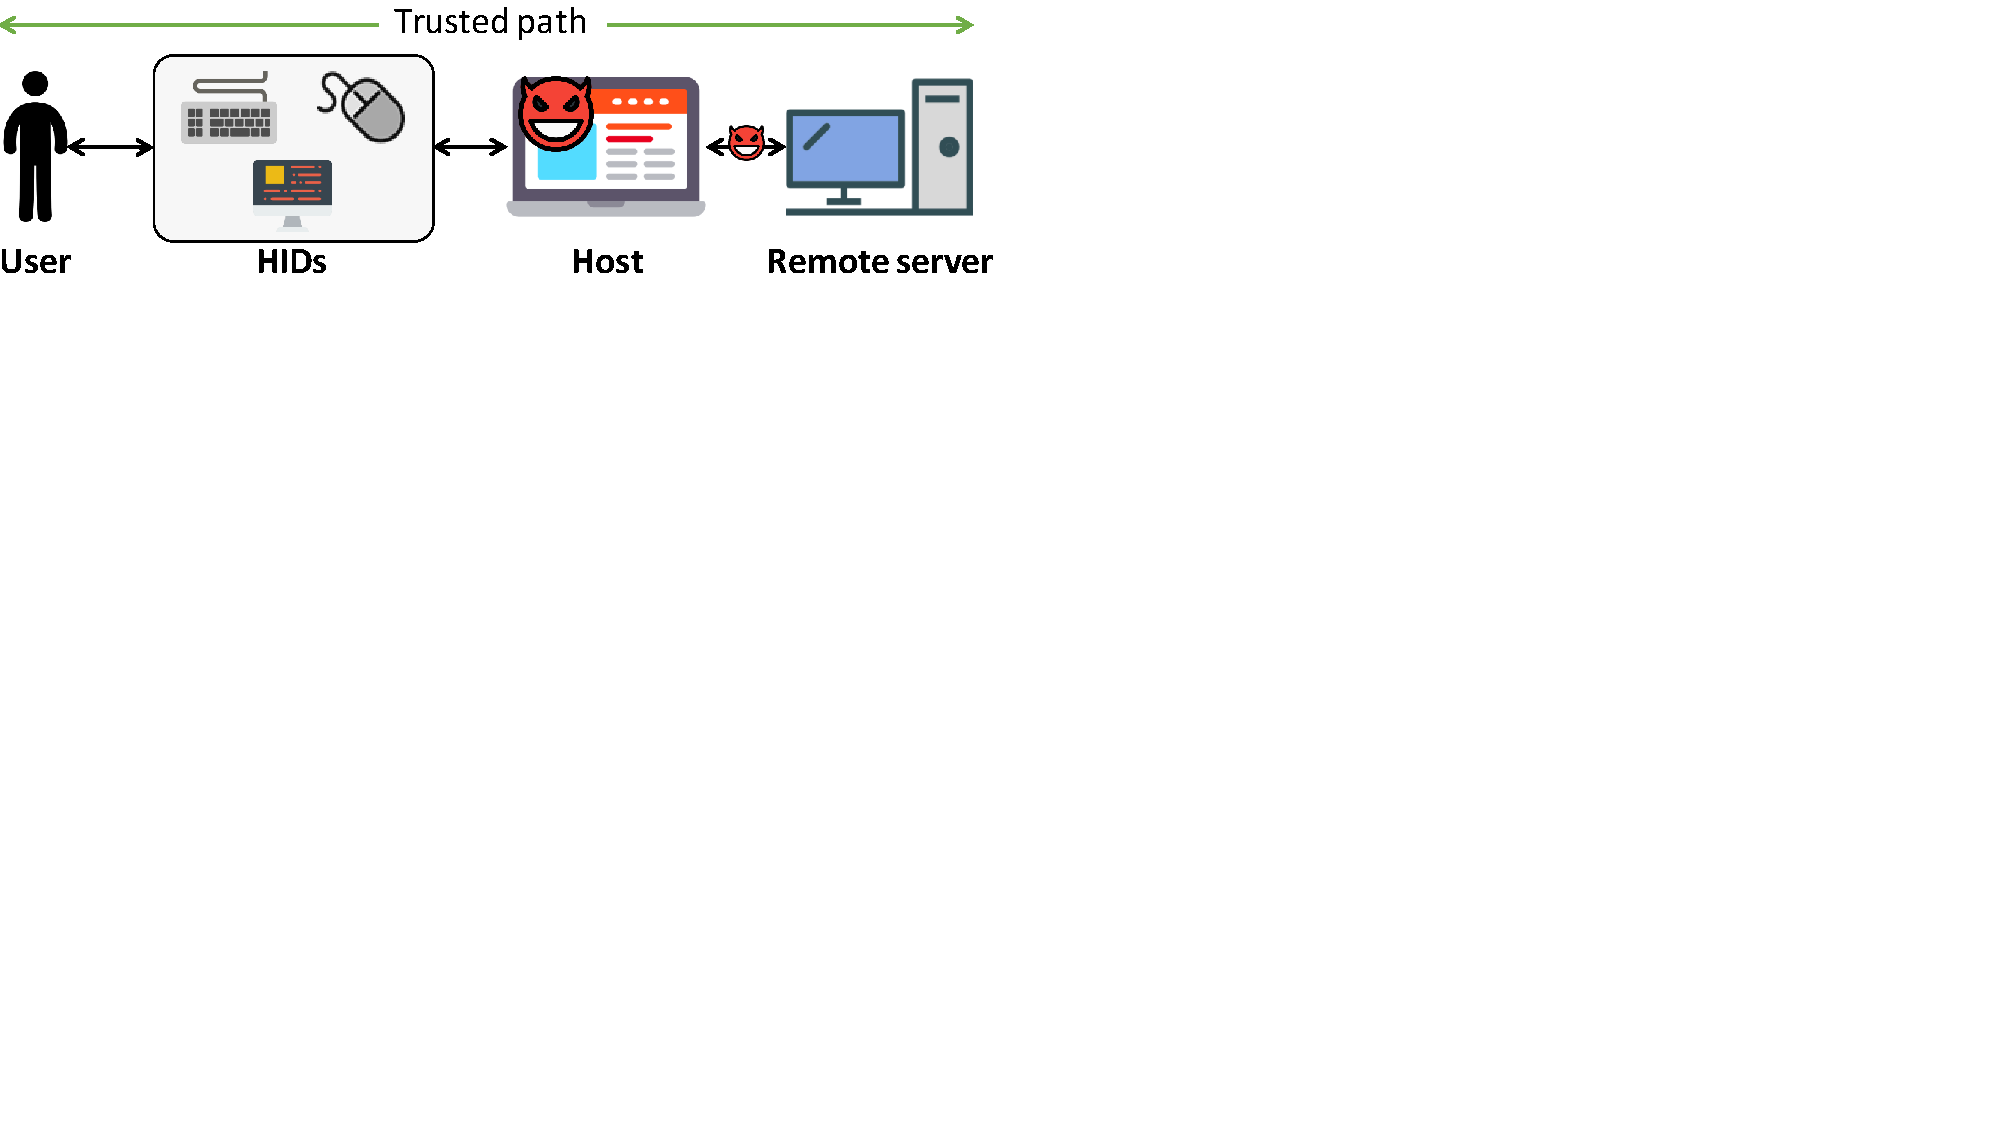
\includegraphics[trim={0 14cm 17cm 0}, clip, width=0.9\linewidth]{systemModel.pdf}
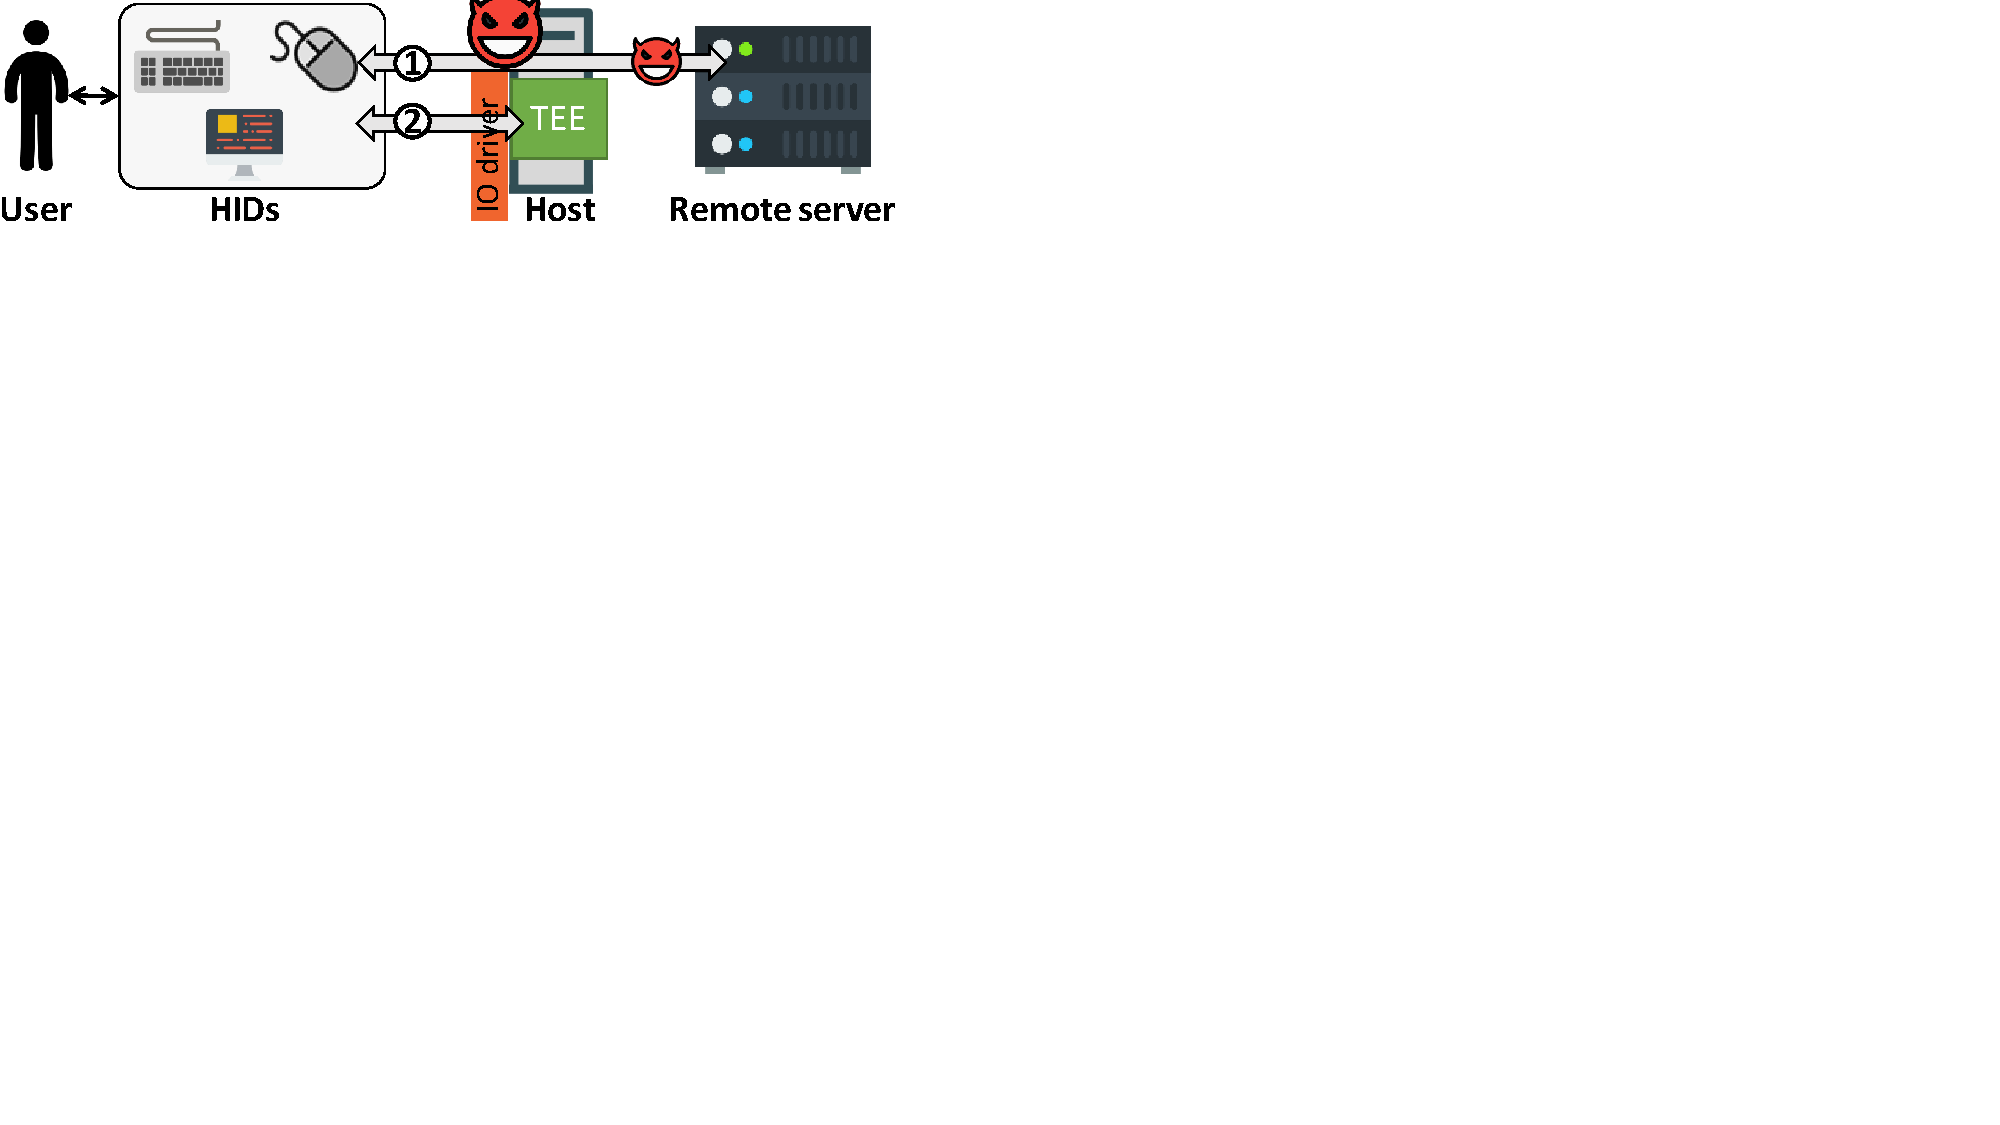
\includegraphics[trim={0 14cm 17cm 0}, clip, width=0.9\linewidth]{systemModel_all.pdf}
\caption{\textbf{Trusted path.} The figures shows the system and the attacker model of the trusted path. We generally consider two trusted path scenarios, \one trusted path to a remote server, and \two trusted path to a trusted execution environment (TEE) such as the Intel SGX.}
\label{fig:trustedPath}
\centering
\end{figure}

A user communicates with a remote server through a computer (we call it host in the rest of the paper), which gives the host access to the plaintext data that goes from the user to the server and vice-versa. Thus, a compromised host can always observe or modify the information exchanged between the user and the server. An adversary that compromises the user's host can alter user intentions, i.e., it can perform arbitrary actions on behalf of the user. Such an adversary is very powerful and difficult to detect or prevent by the remote server. The consequences of such attacks might be severe when safety-critical applications are targeted. The attacker can pass the wrong input to a remote safety-critical system such as a medical device, power plant, etc. 

Trusted execution environments (TEEs) enable remote trust into the code executing on the processor, effectively eliminating the need to trust more significant code base (motherboard, memory modules, OS and other applications). Processor TEE such as Intel SGX relies on the OS to mediate all the user IO. Hence, the problem of isolating user's input and output remains. Therefore, service providers typically operate with the assumption that the data they receive are genuine (generated by the user) and not altered by a compromised host. However, system level TEEs such as ARM TrustZone enables securing the IO data but such mechanism is limited to ARM platforms, making them infeasible for \emph{x86} platforms.%In a few use cases, e.g., online payments, the service providers ask for user confirmation on a second device (phone or specialized hardware) to detect such attacks. However, this solution is limited to applications in which a user can check the input on a secondary device. 

A \emph{Trusted path} provides confidentiality and integrity to the IO data exchanged between the users and the end systems. Figure~\ref{fig:trustedPath} shows two different scenarios where the trusted path extends from user IO devices to : \one a remote server, and \two a local enclave. In principle, a trusted path solves the general security problem of the IO data. 
%But practically establishing a trusted path in general IO devices is a nontrivial problem specifically if one considers the plethora of complex UI objects and input methods as well as different security and functional properties that a solution should satisfy. 
In this paper, we primarily target the trusted path problem to a remote server (such as a remote PLC, web server or remotely accessible medical device etc.).

\iffalse
\subsection{Security Properties}

A \emph{Trusted path} provides confidentiality and integrity to the IO data exchanged between the users and the end systems. In principle, a trusted path solve the general security problem of the IO data. But practically establishing a trusted path in general IO devices is a nontrivial problem specifically if one considers the plethora of complex UI objects and input methods as well as different security and functional properties that a solution should satisfy. We list these properties below. 


\begin{mylist}
  \item \textbf{Input integrity and confidentiality.} These properties define that any input that is coming from the user input devices are fully protected in two ways: i) the input issued by the user reaches to the remote end-point as it was generated by the user - \emph{integrity}, and ii) in specific application scenarios, the attacker-controlled host is entirely oblivious about the input from the user - \emph{confidentiality}. The trusted path system should consider a wide range of input devices, such as keyboard, mouse, touch, etc. We consider any sort of input action by the user that may include moving the mouse or using the keyboard navigation keys to select a specific item in a list.
  
  
  \item \textbf{Output integrity and confidentiality.} Similar to the input integrity, output integrity ensures that information that is sent by the remote endpoint is presented to the user as it was meant to be. One example of output integrity is the integrity of the UI elements. Such property ensures that the host system renders the UI elements faithfully as they were sent by the remote system. Output confidentiality ensures that the information sent by the remote server can not be accessed by the attacker-controlled host. 
  
 %  \item \textbf{Usability.} The trusted path should neither change the typical user interaction with a computer nor should require extensive changes into the existing systems.

  As discussed on the Section~\ref{sec:securityAnalysis}, ensuring output integrity is essential for providing input integrity against advanced attackers that trick the user into sending non-legitimate data to the server. For example, the user wants to send a number \texttt{10} to the server, but the malicious host shows on screen \texttt{100} and fools the user into believing he mistyped a \texttt{0}. The user deletes one \texttt{0} and sees \texttt{10} on the screen---as he intended initially---and submits the data, however, on the server arrives just \texttt{1}. 
  
  Providing output integrity is a challenging task even on systems that have a trusted component that overlays parts of the HDMI frames generated by the untrusted host. Previous works~\cite{huang2012clickjacking} show that when a trusted component and an untrusted one share a screen, the attacker can still manipulate the user to commit unintentional actions to the trusted UI if the system is not designed properly. In our solution we want to guarantee that the user is aware of the UI elements (trusted or untrusted) that she interacts with, therefore preventing related attacks.
  \end{mylist}

\fi




\subsection{Existing Solutions and their drawbacks}

\iffalse
\begin{figure}[t]
\footnotesize
    \centering
    \begin{tikzpicture}[
solved/.style={rectangle,draw,fill=purple!40, rounded corners, align=center},
not/.style={rectangle, draw,fill=orange!60, rounded corners, align=center},
neutral/.style={rectangle, draw, rounded corners, align=center, fill=black!5}
]]
    \node[neutral](root) {Trusted path}
    child { node[neutral, yshift=12pt] (hw) {External\\ HW}}
    child { node[neutral, yshift=8pt, xshift=10pt] (tc) {Transaction\\ confirmation\\ Device}}  
    child { node[neutral, yshift=12pt, xshift=20pt] (tee) {TEE}
      child { node[neutral, yshift=0pt, xshift=-5pt] (teehv) {Hypervisor+\\TEE}}
      child { node[neutral, yshift=0pt, xshift=2pt] (teehw) {TEE + \\ External HW} } }
      child { node[neutral, yshift=8pt, xshift=15pt] (br) {Browser\\ Based}}   
     child { node[neutral, yshift=12pt, xshift=20pt] (hv) {Hypervisor}}  ;
    
    \node[below=0cm of hw] {\textbf{\name}};
    \node[below=0cm of tc] {Uni-dir~\cite{filyanov2011uni}};
    \node[below=0cm of hv] {Overshadow~\cite{Overshadow}};
    \node[below=0cm of teehv] {SGXIO~\cite{weiser2017sgxio}};
    \node[below=0cm of teehw] {Fidelius~\cite{Fidelius}};
     \node[below=0cm of br] {InContext~\cite{blake1998authenticated}};    
    \end{tikzpicture}
    
   \caption{\textbf{Summarization of existing trusted path solutions} by their approach. A detailed description of the related works is discussed in Table~\ref{tab:relatedWorks}.}
     \label{fig:relatedWorksTree}
\end{figure}
\fi

\begin{figure}[t]
\footnotesize
    \centering
    \begin{tikzpicture}[
solved/.style={rectangle,draw,fill=purple!40, rounded corners, align=center},
not/.style={rectangle, draw,fill=orange!60, rounded corners, align=center},
neutral/.style={rectangle, draw, rounded corners, align=center, fill=black!5}
]]
    \node[neutral](root) {Trusted path}
    child { node[neutral, yshift=8pt, xshift=10pt] (tc) {Transaction\\ confirmation Device}}  
    child { node[neutral, yshift=8pt, xshift=80pt] (td) {Trusted Components}
    	child { node[neutral, yshift=0pt, xshift=-40pt] (hw) {External\\ HW}}
    	child { node[neutral, yshift=0pt, xshift=-30pt] (teehv) {Hypervisor+\\TEE}}
      child { node[neutral, yshift=0pt, xshift=-20pt] (teehw) {TEE + \\ External HW}}
      child { node[neutral, yshift=0pt, xshift=-15pt] (br) {Browser\\ Based}}   
     child { node[neutral, yshift=0pt, xshift=-5pt] (hv) {Hypervisor\\ Based}} 
    }	; 
      

    \node[below=0cm of hw] {\textbf{\name}};
    \node[below=0cm of tc] {Uni-dir~\cite{filyanov2011uni}};
    \node[below=0cm of hv] {Overshadow~\cite{Overshadow}};
    \node[below=0cm of teehv] {SGXIO~\cite{weiser2017sgxio}};
    \node[below=0cm of teehw] {Fidelius~\cite{Fidelius}};
     \node[below=0cm of br] {InContext~\cite{blake1998authenticated}};

    
    \end{tikzpicture}
    
   \caption{\textbf{Summarization of existing trusted path solutions} by their approach. A detailed description of the related works is discussed in Table~\ref{tab:relatedWorks} in Appendix~\ref{appendix:sec:summaryResearch}.}
     \label{fig:relatedWorksTree}
\end{figure}


There exist two broad categories of existing solutions that try to solve the problem of trusted paths for IO devices in the presence of a compromised host: A) Solutions where a trusted component that is able to capture user's input/output and then securely mediate it to the destination. The trusted component can be a browser, hypervisor, separate devices, etc., and B) Solutions where unprotected user interaction first happens and then a trusted component is used to double check that manipulation did not happen. %But all of these solutions targeted for different problem settings and models. 
Figure~\ref{fig:relatedWorksTree} provides a board classification of the related works and illustrates where our proposed work stands concerning them. 

\subsubsection{\bfseries Transaction confirmation devices} In their paper, Filyanov et. al~\cite{filyanov2011uni} proposed transaction confirmation device that requires the user to use a separate device to confirm the input parameters. The transaction confirmation suffers from three significant drawbacks. First drawback is risk of\emph{user habituation}. Transaction confirmation device introduces lots of cognitive load over the user and may force the user to confirm their action without even looking to the input data. Second \emph{usability}, i.e., interacting with small device can be cumbersome. Such user action makes the transaction confirmation device impractical in day-to-day interactions. Finally \emph{simple UI}, i.e., transaction confirmation is not practical/suitable for complex interaction, rather simple text-based inputs. 

%In contrary, \name supports generic input devices and supports complex user interfaces and user interactions. Moreover, the complete automated nature of \name does not introduce any cognitive load on the user, making the system less susceptible to user error.


\subsubsection{\bfseries Trusted Execution Environments} TEEs specifically system TEEs such as ARM TrustZone is used in the literature to implement a trusted path between the IO devices and the users. %Several TEEs such as Intel SGX, ARM TrustZone, TPM, Intel TXT, etc. can be used to achieve such functionality.  
VButton~\cite{li2018vbutton} leverages ARM TrustZone to overlay buttons on the mobile device to confirm if the user taps on a specific button. Our solution is fundamentally different from VButtion as i) VButtion is specifically tuned for mobile devices, employing ARM TrustZone whereas our solution is more generic and targets specifically PCs, and ii) mouse input is significantly different than touch-based input as mouse input involves continuous movement where the touch or taps are discrete events. In this paper, we concentrate on the non-specialized hardware platform where compatible TEE technologies such as ARM TrustZone may not be available, e.g., x86 architecture. 
%Intel SGX based trusted path such as BastionSGX~\cite{BASTION-SGX} implements a trusted Bluetooth application inside an Intel SGX enclave to establish a trusted path between the keyboard and mouse and the SGX. But lack of output integrity makes the system unreliable as the paper failed to address how to transfer the mouse data reliably to the user and the remote server. 

\subsubsection{\bfseries Trusted hypervisor/OS-based solutions} Trusted hypervisors and secure micro-kernels are also alternatives to achieve Trusted path. In the work done by Zhou et al.~\cite{zhou2012building}, the authors proposed a generic trusted path on $x86$ systems in pure hypervisor-based design. Solutions such as SGXIO~\cite{weiser2017sgxio}  combine a TEE and a hypervisor to mitigate the shortcomings of TEEs like SGX (i.e., the IO operations are handled by the OS). One major drawback of such solutions is the trust assumption that involves a full hypervisor. One can argue that a hypervisor that provides a rich set of functionalities has code base size of an OS. Second, most of the minimal hypervisor also does not offer common usable features such as rich IO, UI, etc., making them impractical for day-to-day usage. \name avoids such extensive trust assumptions and assumes that the entire host is in control of the attacker.

%There exist several works that use TEE and hypervisor simultaneously to mitigate the shortcomings of TEEs like SGX (i.e., the IO operations are handled by the OS). Existing research such as SGXIO~\cite{weiser2017sgxio} requires the IO drives to be implemented inside the TEE or using trusted hypervisor that extends the size of the TCB significantly. Moreover, TEE requires trust assumption on the processors and additional code bases. One such example is Intel SGX where the trust model includes the physical processor package, SGX SDK, quoting enclave, launch enclave and Intel attestation service. Our proposed solution avoids such extensive trust assumptions and assumes that the entire platform is in control of the attacker.

\subsubsection{\bfseries Browser-based solutions} In their paper InContext, author Huang et al.~\cite{huang2012clickjacking} presents different clickjacking attacks variants and their solution by ensuring context (both temporal and visual) and pointer integrity. The trust model is significantly different from our work as it assumes that the browser and the OS are trusted. This makes the InConext i) not directly compatible with the attacker model that \name targets, and ii) targets a specific attack scenario (clickjacking vs. generic trusted path).



\subsubsection{\bfseries Dedicated hardware-based solution}  Fidelius~\cite{Fidelius} uses raspberry pi's and Intel SGX to create a secure channel between the keyboard and the display device. By doing so, Fidelius provides secure input and display for the character-based device - keyboard. Additionally, Fidelius uses overlays to hide the keyboard input from the compromised host so that the input is only visible to the user. 
%In their work, Brandon et al. ~\cite{brandon2017trusted} demonstrate screen overlay on Android devices using FPGAs. 
None of these works looked into complex user interactions such as mouse movement or complex user interfaces. Fidelius only tackles keyboard-based input and utilizes SGX that separates Fidelius and \name in terms of the trust assumption.  


In summary, even though, there exists a number of research works that look into the problem of trusted path, none of them provide a complete, secure, practical and usable trusted path solution. In our knowledge, \name incorporates all the features together for the first time: complex user interactions and UI elements, generic IO devices and low overhead on the user interactions. All of these are achieved in the smallest trust assumption.  
%Note that the majority of the previous works achieve some form of trusted path specifically for keyboard-based input. However supporting mouse and touch-based input, complex and generic user interfaces and protected users' action (such as the movement of the mouse pointer, gestures, etc.) in a security-sensitive application (such as e-voting) is not a trivial task. Without proper analysis of every frame that the host system produces, it is not possible to track user intention. In our knowledge, our proposed solution is the first to provide such security properties including the confidentiality of user input (e.g., mouse movement). Moreover, we want to achieve this in the absence of any TEE as the trust model of our scenario is significantly different.
Detailed description of the related research is described in Table~\ref{tab:relatedWorks} in Appendix~\ref{sec:summaryResearch}.

\subsection{Goals}
\label{sec:problemStatement:goals}

In the above, we discussed several solutions and research works that solve the problem of constructing a trusted path in different ways. What makes our solution different from them is the specific settings that it targets.\footnote{Is this about threat model or goals?}
%We do not assume trust in the OS, particular drivers, TEEs, hypervisors, etc. As all of these techniques as mentioned earlier require trust on a large code base. Instead, our proposed solution solves the problem of building an efficient, trusted path using an off-the-shelf microcontroller and single board computers that require a bare-minimum trust assumption. The most distinguishing factor is the type of IOs our proposed system targets to protect, namely mouse/touch inputs and sophisticated user interfaces. Existing research works primarily targets character-based input devices such as keyboards, and the methods cannot be trivially applied to mouse/touch-based inputs or complex UI elements. 
The general goals of this paper are the following:

\begin{mylist}
  \item  \textbf{Rich set of IO security features.} Most of the existing trusted path solutions focus on a minimal set of feature (e.g., only support for keyboard). The primary goal of \name is to having compatibility compatible with generic IO device (such as a keyboard, mouse, touch screen, display, etc. in x86 architecture), and to provides a rich set of IO security (such as IO integrity and confidentiality). 
  
  \item  \textbf{Small trust assumption.} Our goal is to provide the aforementioned rich set of IO and security features with minimal trust assumption that does not rely on a specialized hypervisor or trusted OS or TEEs. %Rather \name only trust a plug-and-play small-TCB trusted device that is made out of off-the-shelf components.  
  
  \item \textbf{Usability.} Our goal is also to provide a solution that comes with low deployment overhead such as a plug-and-play device which is compatible with any platform (OS, processor architecture, etc.). Moreover, our goal is not to change the way users interacts with UI elements and imposing no or minimal cognitive load such as eliminating cognitive load that is imposed by transaction confirmation devices, i.e., looking to a security indicator and confirming actions, etc. 

\end{mylist}

In the following section what follow is the \name's design and how \name achieves these goals.


